\documentclass[12pt]{article}

\usepackage{amssymb,amsmath,amsthm}
\usepackage{graphicx}
\usepackage{fullpage}
\usepackage[final,colorlinks,hyperindex,unicode=true]{hyperref}
%\usepackage{tikz}
%\usepackage{pgfplots}
\usepackage[shadow,colorinlistoftodos,textwidth=3cm]{todonotes}



\begin{document}
\thispagestyle{empty}
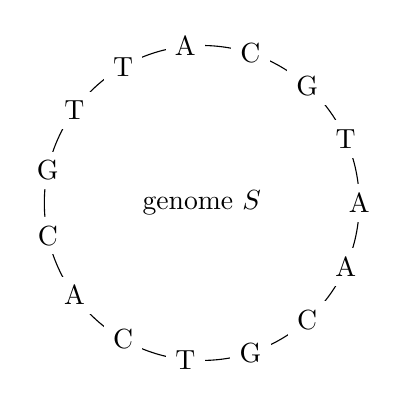
\begin{tikzpicture}
  \draw (0,0) circle (2cm);
  \foreach \i/\a in {0/A,1/T,2/G,3/C,4/A,5/T,6/T,7/G,8/C,9/A,10/C,11/T,12/G,13/C,14/A} {
    \node[fill=white] at (360*\i/15:2cm) {\a};
  }
  \node at (0,0) {genome $S$};




\end{tikzpicture}
\end{document}
